\documentclass{article}
% --- Packages ------------------------------------------- ----- Standard Packages --------------------------------
\usepackage{graphicx} % Required for inserting images
\usepackage{amsthm} %let us define theorems
\newtheorem{theorem}{Theorem}
\usepackage{amssymb} %Useful Symbols
\usepackage{mathtools} %better version of amsmath
\usepackage{microtype} %make things look nicer
\usepackage{float} %Let figures appear the right place on page
\usepackage{scalerel}
\usepackage{caption}
\usepackage{subcaption}
\usepackage{hyperref}
% https://tex.stackexchange.com/questions/254044/caption-and-label-on-minted-code
\usepackage[newfloat]{minted}
\usepackage{caption}
\newenvironment{code}{\captionsetup{type=listing}}{}
\SetupFloatingEnvironment{listing}{name=Code Block}
% --- Style for haskell code
\usepackage{listings}
\lstset{
  frame=none,
  xleftmargin=2pt,
  stepnumber=1,
  numbers=left,
  numbersep=5pt,
  numberstyle=\ttfamily\tiny\color[gray]{0.3},
  belowcaptionskip=\bigskipamount,
  captionpos=b,
  escapeinside={*'}{'*},
  language=haskell,
  tabsize=2,
  emphstyle={\bf},
  commentstyle=\it,
  stringstyle=\mdseries\rmfamily,
  showspaces=false,
  keywordstyle=\bfseries\rmfamily,
  columns=flexible,
  basicstyle=\small\sffamily,
  showstringspaces=false,
  morecomment=[l]\%,
}
% ---- bibliography ----
\usepackage[backend = biber, style = alphabetic, urldate = long]{biblatex}
\bibliography{References.bib}
% ----- custom commands ----
%\newcommand{\ors}{\overline{\text{rs}}}
%\newcommand{\rs}{\text{rs}}
%\newcommand{\oas}{\overline{\text{as}}}
%\newcommand{\xo}{\overline{\text{x}}}
%\newcommand{\as}{\text{as}}
\newcommand{\ors}{\overline{rs}}
\newcommand{\obs}{\overline{bs}}
\newcommand{\ob}{\overline{b}}
\newcommand{\rs}{rs}
\newcommand{\xs}{xs}
\newcommand{\oas}{\overline{as}}
\newcommand{\xo}{\overline{xs}}
\newcommand{\as}{as}
\newcommand{\bs}{bs}
\newcommand{\cs}{cs}
\newcommand{\ds}{ds}
\title{Scan Reverse-AD Improvements applied to the Futhark Compiler}
\author{Peter Adema (qlz919@alumni.ku.dk)\\
Sophus Valentin Willumsgaard (hwx333@alumni.ku.dk)}
\date{\today}

\begin{document}

\maketitle
\tableofcontents
\section{Introduction}
The purpose of this project is to implement the algorithm given in \cite{PPAD}, for reverse
automatic differentiation of the scan operator in Futhark.
In this report,
we describe the procedure for reverse automatic differentiation of a
scan operation given in \cite{PPAD},
and how it differs from the current implementation as described in
\cite{Futhark}.
We then show how we have implemented the procedure in the Futhark compiler,
and lastly give benchmarks to compare with the current implementation.
\section{Description of Algorithm}
We here give a description of the general-case procedures for automatic differentiation of
scan described in \cite{PPAD} and \cite{Futhark}.

We will use \(\odot\) to denote a general associative operator defined
either on \(\mathbb{R}\) or \(\mathbb{R}^{n}\) which is differentiable in each variable,
and which have a neutral element \(e_{\odot}\).
Given an array of variables \(\xs\),
we let \(\xo\) denote the array of adjoint values in AD.
Following \cite{PPAD},
and the current implementation of AD in Futhark,
we let the adjoint values have the same type as their corresponding variables.
For an array \(as\),
we switch between the notation \(as[i]\) and \(as_{i}\) to denote its elements
depending on the context.

\subsection{Non-Parallel Procedure}
Assuming we have a program containing the following definition
\begin{minted}[escapeinside=||]{futhark}
let |$\rs$| = scan |$\odot$| |$e_{\odot}$| |$\as$|
\end{minted}
our task is to use the values of
\(\ors, \rs, \as\) to calculate \(\oas\).
From the definition of scan, we have
\begin{align*}
	\rs[0] = \as[0] \\
	\rs [i+1] = \rs[i] \odot \as[i+1]
\end{align*}
We see that the value of \(\rs[i]\) depend on \(\rs[j]\) for \(i>j\).
For this reason we introduce another array of adjoint vectors \(\xo\),
which is similar to \(\ors\), but also includes the contribution of the lower
indices upon the higher ones.
From the above formulas we then get
\begin{align*}
	\xo [n-1] = \ors [n-1]     \\
	\xo [i-1] = \frac{\partial (\rs [i-1] \odot \as[i])}{\partial \rs[i-1]}
	\cdot \xo[i]   + \ors[i-1] \\
	\oas [0] = \xo[0]          \\
	\oas [i] = \frac{\partial (\rs [i-1] \odot \as[i])}{\partial \as[i]}
	\cdot
	\xo[i]
\end{align*}
From these formulas, we can calculate \(\oas\) in two loops.
The first loop inductively calculates \(\xo\),
and the second loop calculate \(\oas\),
however this would not preserve parallelism. We will now describe how to
calculate these in a parallel way.
\subsection{Parallelization}
We note that the calculation of \(\oas[i]\) does not depend on any values of
\(\oas\),
so it can be calculated by applying a map operator,
preserving parallelization.

The harder challenge is then to calculate \(\xo\).
To resolve this,
we define a new monoid structure \(\otimes\) on \((\mathbb{R}^{n})^{3}\)
given by

\begin{align*}
	[r_{1}, a_{1}, \overline{r}_{1}] \otimes
	[r_{2}, a_{2}, \overline{r}_{2}] =
	\left[r_{1}, a_{1} \otimes a_{2},
		\frac{\partial (r_{1} \odot a_{1})}{\partial r_{1}} \cdot \overline{r}_{2} + \overline{r}_{1} \right]
\end{align*}
in \cite{PPAD} they show this operator is associative and have a right
identity \(e_{\otimes} :=[e_{\odot}, e_{\odot}, 0]\).

\begin{theorem}
	The following procedure
	\begin{minted}[escapeinside=££]{futhark}
let £$ms$£ = zip3 £$\rs$£ (tail £$\as$£ ++ £$e_{\odot}$£) £$\ors$£
let (£$\bs,\cs,\ds$£) = scan_right £$\otimes$£ £$e_{\otimes}$£ £$ms$£ |> unzip3
in ds
\end{minted}
	calculates \(\xo\).
\end{theorem}
\begin{proof}
	The argument follows by reverse induction on indices of \(\xo\).
	Starting with \(n-1\), we have
	\begin{align*}
		\ds_{n-1} = \ors_{n-1}
	\end{align*}
	which agrees with  \(\xo_{n-1}\).
	Now assuming that \(\ds_{i} = \xo_{i}\) we have
	\begin{align*}
		[\bs_{i-1}, \cs_{i-1}, \ds_{i-1}] \\
		= [\rs_{i-1}, \as_{i}, \ors_{i-1}]\otimes
		[\bs_{i}, \cs_{i}, \ds_{i}]       \\
		= \left[\rs_{i-1}, a_{i} \otimes \cs_{i},
			\frac{\partial (rs_{i-1} \odot a_{i})}{\partial r_{i-1}} \cdot \ds_{i} + \ors_{i-1}
		\right]                           \\
		= \left[\rs_{i-1}, a_{i} \otimes \cs_{i},
			\frac{\partial (rs_{i-1} \odot a_{i})}{\partial r_{i-1}} \cdot \xo_{i} + \ors_{i-1}
			\right]
	\end{align*}
	We then see that the third argument agrees with our formula for
	\(\xo_{i-1}\) above, finishing the induction argument.
\end{proof}
Given the definition of \(\otimes \), we can then calculate \(\oas\) by
\begin{minted}[escapeinside=££]{futhark}
let £$ms$£ = zip3 £$\rs$£ (tail £$\as$£ ++ [£$e_{\odot}$£]) £$\ors$£
let (£$\bs,\cs,\ds$£) = scan_right £$\otimes$£ £$e_{\otimes}$£ £$ms$£ |> unzip3
in map3 (\x y z -> £$\partial (x \odot y)/\partial y \cdot z$£) ([£$e_{\odot}$£] ++ init £$\rs$£ ) £$ \as $£ £$ \ds $£
\end{minted}
Where the last line correspond to a use of vjp
\begin{minted}[escapeinside=££]{futhark}
map3 (\x y z -> vjp (\w -> £$x\odot w$£) y z) ([£$e_{\odot}$£] ++ init £$\rs$£ ) £$ \as $£ £$ \ds $£
\end{minted}
\subsection{Comparison to current Futhark implementation}
The general idea for reverse AD of scan operators in the current Futhark
implementation,
is similar to the above procedure,
in that it first uses a scan for calculating \(\xo\),
followed by a map for \(\oas\).
The map for \(\oas\) is exactly the same,
but the calculations of \(\xo\) differs.

Instead of calculating the derivatives
\begin{align*}
	\frac{\partial rs[i-1] \odot \as[i]}{\partial \as[i]}
\end{align*}
inside the scan,
the Jacobians representing the derivative functions are instead calculated
first, and stored to be used in the scan.
This can be done by a map operator,
since the derivative only depend on \(\rs, \as\) and the operator \(\odot\).
From this, \(\xo\) can be calculated by a scan operator.

It is also worth noting that in special cases,
such as then the operator \(\odot\) is addition or a vectorised version of scalar operator,
there are more optimal ways of calculating the adjoint values,
which the compiler takes advantage of.
\subsection{Discussion about Efficiency}
The disadvantages of calculating the Jacobians beforehand,
is that it is memory-intensive to have so much data to be used inside the
scan operator. Furthermore calculating the Jacobians seperated from their
application to the adjoints,
removes the possibility of using optimization built in the automatic
differentiation.
For example if the adjoint values are 0 in some dimensions,
the derivatives does not need to be calculated in those dimensions.

However calculating the Jacobian beforehand has some advantages. In
particular,
the current Futhark compiler after calculating the Jacobian, performs static
analysis to see if the Jacobian is of block-diagonal form.
In this case the Jacobians can be represented by much smaller matrices,
which greatly optimises the scan step in computation.
The scan is also harder to optimize compared to the map,
so when the operator inside the scan is more complicated as it is in the
\cite{PPAD} implementation,
it will cause a greater runtime.
\newpage
\section{Implementation}
The implementation of the algorithm described in \cite{PPAD} was driven by the \href{https://github.com/diku-dk/ifl23-revad-red-scan/blob/main/scan/scan-adj-comp.fut}{reference implementation} in Futhark code from \cite{Futhark}, with the structure of the compiler code globally following the Futhark reference code. There is one notable difference between the Futhark implementation and the compiler code, namely in the treatment of neutral elements for \lstinline{op_lifted}. In \cite{PPAD} it was noted that for the lifted operator as defined there, \lstinline{(e, e, 0)} would serve as a right-neutral element, allowing for a reverse-scan over the constructed array \lstinline{m} (with \lstinline{e} being the original neutral element). This approach leads to the simple definition of \lstinline{op_lift} from the Futhark reference code in Code Block \ref{code:fut-oplift}:
\begin{code}
	\begin{minted}[linenos]{futhark}
let z_term = op_bar_1 op (x1, a1, y2_h)
let z = plus z_term y1_h
in  (x1, op a1 a2, z)
\end{minted}
	\caption{Reference Futhark code for \lstinline{op_lift} (operator for scan calculating adjoints for scan intermediates rs/xs). \lstinline{op_bar_1} refers to differentiating \lstinline{op} with respect to its first argument.\\}
	\label{code:fut-oplift}
\end{code}
We can similarly define the core operator in the compiler code, as shown in Code Block \ref{code:hsk-oplift}:
\begin{code}
	\begin{minted}[linenos]{haskell}
op_lift px1 pa1 py1 pa2 py2 adds = do
    op_bar_1 <- mkScanAdjointLam ops (scanLambda scan) 
                    WrtFirst (Var . paramName <$> py2)
    let op_bar_args = toExp . Var . paramName <$> px1 ++ pa1
    z_term <- map resSubExp <$> eLambda op_bar_1 op_bar_args
    let z =
        mapM
          (\(z_t, y_1, add) -> head <$> eLambda add [toExp z_t, toExp y_1])
          (zip3 z_term (Var . paramName <$> py1) adds)
    
    let x1 = subExpsRes <$> mapM (toSubExp "x1" . Var . paramName) px1
    op <- renameLambda $ scanLambda scan
    let a3 = eLambda op (toExp . paramName <$> pa1 ++ pa2)
    
    concat <$> sequence [x1, a3, z]
\end{minted}
	\caption{Haskell code for \lstinline{op_lift} (operator for scan calculating adjoints for scan intermediates rs/xs).\\}
	\label{code:hsk-oplift}
\end{code}
However, while the above is an accurate translation of the Futhark reference code, ensuring that it produces correct results under a scan required more work. This is due to that the constant folding mechanism in later passes of the Futhark compiler occasionally made incorrect inferences regarding how the neutral element could be inlined in the scan. As a concrete example, when differentiating \lstinline{scan f32.max f32.lowest}, the IR generated for \lstinline{op_bar_1} would look like Code Block \ref{code:ir-wrong}:

\begin{code}
	\begin{minted}[linenos]{rust}
// This lambda is op_lift for f32.max, as an argument to scanomap
 \ {...,
    a1 : f32,
    y1_h : f32,
    y2_h: f32
    ...} : {..., f32} ->
        let {convop_x_7531 : bool} =
          le32(a1, -f32.inf) // x1 was replaced with the n.e.
        let {convop_x_7532 : i32} =
          btoi bool convop_x_7531 to i32
        let {der_x1 : f32} =
          sitofp i32 convop_x_7532 to f32
        let {z_term : f32} =
          fmul32(y2_h, der_x1)
        ...
        let {z : f32} =
          fadd32(y1_h, z_term)
        in {..., z}
\end{minted}
	\caption{Incorrect IR for \lstinline{op_bar_1}. Names have been changed for clarity.\\}
	\label{code:ir-wrong}
\end{code}
\vspace{0.3cm}
We can see that the original intention of Line 8 in Code Block \ref{code:ir-wrong} would have been to check if $a_1 \leq x_1$, as in that case the carry $x_1$ would have continued through the \lstinline{f32.max}, adding the contribution of \lstinline{y2_h} to \lstinline{z} in the form of \lstinline{z_term}. However, we can see that, during optimization of the generated function, $x_1$ was replaced with the constant value from the neutral value (\lstinline{f32.lowest} is \lstinline{-f32.inf}).

To mitigate this, the method we found was to add an extra boolean field to all elements of the scan, which would be \lstinline{True} for the neutral element and \lstinline{False} for all elements from the real array. Modifying \lstinline{op_lift} such that it ignored neutral elements and only performed the calculations when both of its arguments were non-neutral elements added overhead to the operator, but prevented the incorrect inlining from taking place. Notably, adding this check to only one side (i.e. only guarding against neutral elements as a first argument) fixed some instances of incorrect inlining (such as \lstinline{scan f32.max}, and even though the reverse scan makes it such that neutral elements should only appear as second argument), but generated new failures as well (causing the scan of matrix multiplication to fail). As such, a guard against neutral elements was necessary on both sides.

Using this implementation of \lstinline{op_lift} (named \lstinline{mkPPADOpLifted} in the compiler code), we proceeded to implement the main body of the scan reverse-AD. Code Block \ref{code:fut-scanbar} shows the reference code for this (named \lstinline{scan_bar}):
\newpage
\begin{code}
	\begin{minted}[linenos]{futhark}
let ys = scan op e u
let as_lft = map (\i -> if i < n-1 then u[i+1] else e) (iota n)
let m = zip3 ys as_lft x_b
let (_, _, rs_adj) = unzip3 <|
    scan_right (op_lft plus op) (e, e, zero) m
let ys_right = map (\i -> if i == 0 then e else ys[i-1]) (iota n)
let as_bar = map (op_bar_2 op) (zip3 ys_right u rs_adj)
in  as_bar
\end{minted}
	\caption{Reference Futhark code for \lstinline{scan_bar} (main reverse AD fuction).}
	\label{code:fut-scanbar}
\end{code}
\vspace{0.3cm}
The compiler code is very similar in structure, with the exception of the additional boolean field marking the neutral element as "e" and the original array as "not e". The following Code Block \ref{code:hsk-scanbar} was added as part of the main \lstinline{diffScan} function (each line grouping is one \lstinline{let} from Code Block \ref{code:fut-scanbar}):
\begin{code}
	\begin{minted}[linenos]{haskell}
let e = scanNeutral scan
as_lift <- asLiftPPAD as w e

isnt_e <- letExp "isnt_e" $ BasicOp $ Replicate (Shape [w]) $ Constant $ BoolValue False
let m = ys ++ as_lift ++ ys_adj ++ [isnt_e]

op_lft <- mkPPADOpLifted ops as scan w
a_zero <- mapM (fmap Var . letExp "rscan_zero" . zeroExp . rowType) as_types
let lft_scan = Scan op_lft $ e ++ e ++ a_zero ++ [Constant $ BoolValue True]
rs_adj <- (!! 2) . chunk d <$> scanRight m w lft_scan

ys_right <- ysRightPPAD ys w e

op_bar_2 <- finalMapPPAD ops as scan
letTupExp "as_bar" $ Op $ Screma w (ys_right ++ as ++ rs_adj) $ mapSOAC op_bar_2
\end{minted}
	\caption{Haskell code for \lstinline{scan_bar} (main reverse AD fuction). \lstinline{w} is the length of the arrays in \lstinline{as}.\\}
	\label{code:hsk-scanbar}
\end{code}
\vspace{0.3cm}
The functions \lstinline{asLiftPPAD}, \lstinline{scanRight}, \lstinline{ysRightPPAD} and \lstinline{finalMapPPAD} were also added in the compiler implementation, all bearing close resemblance to the reference implementation in terms of structure.

Finally, we would like to remark that in some cases, the utility function \lstinline{lambdaReturnType} gave element types instead of the true returns types; returning \lstinline{f32} when a lambda actually returned \lstinline{[]f32}. While there was a relatively simple workaround for this bug, it should be noted that these incorrect types currently cause compilation errors in the 'normal' scan reverse-AD compiler (see \href{https://gist.github.com/p-adema/c8fc4fd5823baca18d90385370aeda5d}{this gist}).

\newpage
\section{Benchmark}
We have performed benchmarks for different operations,
to compare the efficiency of our implementation with the current implementation in Futhark.

\subsection{Methodology}
\subsubsection*{Operators}
Our choice of operators to apply scan to are very similar to the ones given
in \cite{Futhark}, so we are able to compare the results.
These operators are
\begin{enumerate}

	\item addition, multiplication and min.
	\item vectorised addition and multiplication.
	\item Two linear operators given by
	      \begin{align*}
		      (x_{0},y_{0}) \odot (x_{1},y_{1})
		      =
		      (x_{1} + y_{1}\cdot x_{0}, y_{0}\cdot y_{1}) \\
		      (x_{0},y_{0}) \odot' (x_{1},y_{1})
		      =
		      (x_{0} + x_{1} + y_{0}\cdot y_{1}, y_{0}+ y_{1})
	      \end{align*}
	\item matrix multiplication for matrices of size 2x2, 3x3 and 5x5.
\end{enumerate}
We have further added a non-linear operator
\begin{align*}
	(x_{0},y_{0}, z_{0}) \otimes (x_{1},y_{1}, z_{1})
	=
	(x_{0}^{\ln x_{1}},y_{0}\cdot y_{1}, z_{0}+z_{1})
\end{align*}
with identity \((e,1,0)\).
\subsubsection*{Datasets}
For each operation we run two tests with randomly generated arrays of f32
floats.
\begin{itemize}
	\item For vectorised multiplication and addition we have arrays of
	      dimensions \(16 \times 10^{7}\) and \(16 \times 10^{8}\).
	\item For 5x5 matrix multiplication, we have two arrays of dimensions \(25 \times 10^{7}\)
	      and \(25 \times 2 \times 10^{7}\).
	\item For 3x3 matrix multiplication, we have two arrays of dimensions \(9 \times 10^{7}\)
	      and \(9 \times 10^{8}\).
	\item For 2x2 matrix multiplication, we have two arrays of dimensions \(4 \times 10^{7}\)
	      and \(4 \times 10^{8}\).
	\item For the other operations we have two arrays of dimensions
	      \(10^{7}\) and \(10^{8}\).
\end{itemize}
Further for 3x3 matrix multiplication and the second linear operator \(\odot'\),
we have added more datasets, for generating the graphs in \ref{graph1}
and \ref{graph2}.
\subsubsection*{Hardware}
We ran the benchmarks on the Futhark machine hendrixfut01fl in the Hendrix
cluster,
which is equipped with a Nvidia A100 GPU.
\subsubsection*{Software}
In our benchmarks, we test 4 different implementations.
\begin{enumerate}
	\item Our own implementation \textbf{PPAD-C} of the \cite{PPAD} in the Futhark compiler.
	\item An implementation of the same algorithm in Futhark \textbf{PPAD-F} written by Cosmin
	      for benchmarking for the \cite{Futhark} paper.
	      This is to compare how efficient our implementation of the algorithm is.
	\item The current implementation \textbf{RMAD} in Futhark,
	      so we can compare the two different procedures.
	\item The primal code, which performs the scan operation without any AD,
	      to measure the AD overhead.

\end{enumerate}





\begin{figure}[h]
	\makebox[\textwidth][c]{
		\begin{tabular}{|c|c c c c|c|c c c c|}
			\hline
			MM5x5     & Primal & RMAD   & PPAD-C & PPAD-F & MM3x3     & Primal & RMAD  & PPAD-C & PPAD-F \\
			\hline
			\(D_{1}\) & 7616   & 33828  & 170336 & 45008  & \(D_{1}\) & 960    & 6566  & 8263   & 6198   \\
			\(D_{2}\) & 37626  & 167955 & 848794 & 223939 & \(D_{2}\) & 8986   & 64790 & 81734  & 61005  \\
			\hline
			MM2x2     & Primal & RMAD   & PPAD-C & PPAD-F & LO        & Primal & RMAD  & PPAD-C & PPAD-F \\
			\hline
			\(D_{1}\) & 370    & 1552   & 2086   & 1579   & \(D_{1}\) & 188    & 614   & 750    & 746    \\
			\(D_{2}\) & 3360   & 15019  & 20264  & 15101  & \(D_{2}\) & 1552   & 5637  & 6984   & 6698   \\
			\hline
			LO2       & Primal & RMAD   & PPAD-C & PPAD-F & NLO       & Primal & RMAD  & PPAD-C & PPAD-F \\
			\hline
			\(D_{1}\) & 190    & 773    & 641    & 631    & \(D_{1}\) & 479    & 1376  & 2133   & 1721   \\
			\(D_{2}\) & 1560   & 7228   & 5919   & 5647   & \(D_{2}\) & 4343   & 12891 & 20227  & 15592  \\
			\hline
			Add       & Primal & RMAD   & PPAD-C & PPAD-F & VAdd      & Primal & RMAD  & PPAD-C & PPAD-F \\
			\hline
			\(D_{1}\) & 144    & 147    & 215    & 157    & \(D_{1}\) & 1449   & 302   & 10265  & 1263   \\
			\(D_{2}\) & 784    & 1270   & 1848   & 1325   & \(D_{2}\) & 12995  & 2608  & 91315  & 11537  \\
			\hline

			Min       & Primal & RMAD   & PPAD-C & PPAD-F & Mul       & Primal & RMAD  & PPAD-C & PPAD-F \\
			\hline
			\(D_{1}\) & 146    & 147    & 215    & 565    & \(D_{1}\) & 106    & 368   & 479    & 476    \\
			\(D_{2}\) & 1183   & 1270   & 1848   & 4866   & \(D_{2}\) & 783    & 3229  & 4323   & 4012   \\
			\hline
		\end{tabular}
	}
	\makebox[\textwidth][c]{
		\begin{tabular}{|c|c|c|c|c|}
			VMul      & Primal & RMAD & PPAD-C & PPAD-F \\
			\hline

			\(D_{1}\) & 1448   & 716  & 23582  & 24147  \\
			\(D_{2}\) & 12968  & 6558 & 214282 & 214121 \\
			\hline
		\end{tabular}}
	\caption{The results of the benchmark. The results are the runtime of each
		benchmark measured in \(\mu s\)}
	\label{results}
\end{figure}
\begin{figure}[h]
	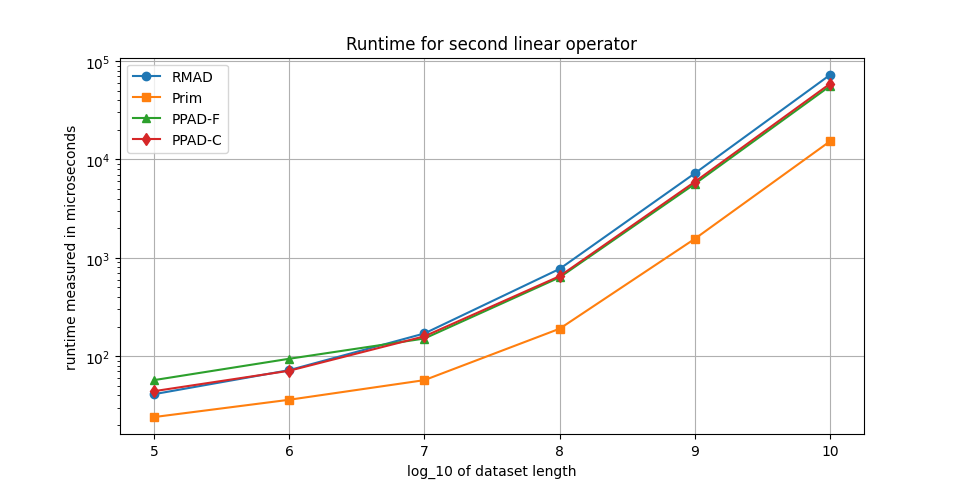
\includegraphics[width=\textwidth]{graphofruntime.png}
	\caption{Graph of results for Second linear operator \(\odot'\).}
	\label{graph1}
\end{figure}
\begin{figure}[h]
	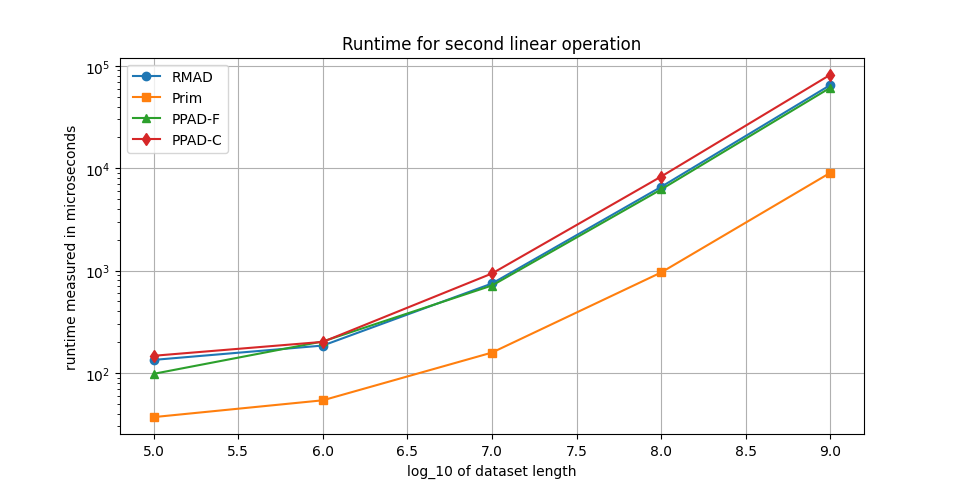
\includegraphics[width=\textwidth]{graphofruntime2.png}
	\caption{Graph of results of matrix multiplication for 3x3 matrices.}
	\label{graph2}
\end{figure}
\subsection{Results}
The results can be seen in figures \ref{results},
\ref{graph1} and
\ref{graph2}.
\subsubsection*{Comparison of PPAD implementation in Futhark and compiler}
Comparing the two PPAD implementations,
we see that the compiler implementation runs slower or equal in 10/11 benchmarks,
but that for 9 out of 11 benchmarks the runtime is at most double the
runtime of the Futhark implementation.

The two exceptions to these are the matrix Multiplication for 5x5 matrices,
and the vectorised addition,
suggested the code can still be optimised for datatypes consisting of
arrays.
This is however contrasted by the vectorised multiplication which performs
equally well in both implementations.

\subsubsection*{Comparison between PPAD and RMAD procedure}
We see that PPAD-compiler implementation performs worse than the RMAD
implementation, in all cases except for the second linear operator \(\odot'\).

In a lot of cases this is expected as the vectorised operations, have extra
optimization in \cite{Futhark}, making them run faster.
We still however see that slowdown is no more than a factor 2, for all
benchmarks except 5x5 matrix multiplication, but that seems to an issue with
the compiler implementation, rather than the procedure itself, as the
futhark implementation is much close to the RMAD procedure.

\subsubsection*{Comparison to primal code}
Overall it seems all 3 of the implementations are not the far from each
other compared to the primal code as seen in \ref{graph1}
and
\ref{graph2},
except for the cases where the compiler is optimized to that particular
operation as in Add, VAdd and VMul.
This suggest that optimizing the AD for specific
operations when applicable, can be profitable way to achieve higher
efficiency.
\section{Conclusion}
We suspect that the cause for the lacking performance in our compiler-generated version of the PPAD
algorithm lies in the additional checks for neutral elements that are inserted around
every call to \lstinline{op_lifted}, but verification of this would require a correct
compiler implementation without these checks.

In conclusion, using the PPAD algorithm as an alternative for the current implementation in the
Futhark compiler holds promise, but due to practical limitations and lacking performance, further
work would need to be done to make it a viable alternative in terms of performance.
\printbibliography
\end{document}
